%%%%%%%%%%%%%%%%%%%%%%%%%%%%%%%%%%%%%%%%%
% Beamer Presentation
% LaTeX Template
% Version 1.0 (10/11/12)
%
% This template has been downloaded from:
% http://www.LaTeXTemplates.com
%
% License:
% CC BY-NC-SA 3.0 (http://creativecommons.org/licenses/by-nc-sa/3.0/)
%
%%%%%%%%%%%%%%%%%%%%%%%%%%%%%%%%%%%%%%%%%

%----------------------------------------------------------------------------------------
%	PACKAGES AND THEMES
%----------------------------------------------------------------------------------------

\documentclass[aspectratio=169]{beamer}

\mode<presentation> {

 
% The Beamer class comes with a number of default slide themes
% which+++ change the colors and layouts of slides. Below this is a list
% of all the themes, uncomment each in turn to see what they look like.

%\usetheme{default}
%\usetheme{AnnArbor}
%\usetheme{Antibes}
%\usetheme{Bergen}
%\usetheme{Berkeley}
%\usetheme{Berlin}
%\usetheme{Boadilla}
%\usetheme{CambridgeUS}
%\usetheme{Copenhagen}
%\usetheme{Darmstadt}
%\usetheme{Dresden}
%\usetheme{Frankfurt}
%\usetheme{Goettingen}
%\usetheme{Hannover}
%\usetheme{Ilmenau}
%\usetheme{JuanLesPins}
%\usetheme{Luebeck}
\usetheme{Madrid}
%\usetheme{Malmoe}
%\usetheme{Marburg}
%\usetheme{Montpellier}
%\usetheme{PaloAlto}
%\usetheme{Pittsburgh}
%\usetheme{Rochester}
%\usetheme{Singapore}
%\usetheme{Szeged}
%\usetheme{Warsaw}

% As well as themes, the Beamer class has a number of color themes
% for any slide theme. Uncomment each of these in turn to see how it
% changes the colors of your current slide theme.

%\usecolortheme{albatross}
%\usecolortheme{beaver}
%\usecolortheme{beetle}
%\usecolortheme{crane}
%\usecolortheme{dolphin}
%\usecolortheme{dove}
%\usecolortheme{fly}
%\usecolortheme{lily}
%\usecolortheme{orchid}
%\usecolortheme{rose}
%\usecolortheme{seagull}
%\usecolortheme{seahorse}
%\usecolortheme{whale}
%\usecolortheme{wolverine}

%\setbeamertemplate{footline} % To remove the footer line in all slides uncomment this line
%\setbeamertemplate{footline}[page number] % To replace the footer line in all slides with a simple slide count uncomment this line

\definecolor{UOSred}{rgb}{0.6745098039215686, 0.02352941176470588, 0.2039215686274510} % UBC Blue (primary)
\definecolor{UOSgrey}{rgb}{0.8117647058823529, 0.8117647058823529, 0.8117647058823529} % UBC Grey (secondary)

\setbeamercolor{palette primary}{bg=UOSred,fg=white}
\setbeamercolor{palette secondary}{bg=UOSred,fg=white}
\setbeamercolor{palette tertiary}{bg=UOSred,fg=white}
\setbeamercolor{palette quaternary}{bg=UOSred,fg=white}
\setbeamercolor{structure}{fg=UOSred} % itemize, enumerate, etc
\setbeamercolor{section in toc}{fg=UOSred} % TOC sections

%gets rid of bottom navigation bars
\setbeamertemplate{footline}[frame number]{}

%gets rid of bottom navigation symbols
\setbeamertemplate{navigation symbols}{}


\usepackage{amsmath}
\usepackage{selinput}      % Halbautomatische Auswahl der Eingabecodierung
\SelectInputMappings{      % mit Hilfe ausgewählter Glyphen
  adieresis={ä},	   % siehe: http://partners.adobe.com/public/developer/en/opentype/glyphlist.txt
  germandbls={ß},
  Euro={€}
}

\addtobeamertemplate{footline}{%
  \leavevmode%
  \hbox{%
  \begin{beamercolorbox}[wd=\paperwidth,ht=2.25ex,dp=1ex,center]{author in head/foot}%
     \insertsectionnavigationhorizontal{\paperwidth}{}{}
  \end{beamercolorbox}}%

}

% Override palette coloring with secondary
\setbeamercolor{subsection in head/foot}{bg=UOSgrey,fg=white}

%\setbeamertemplate{navigation symbols}{} % To remove the navigation symbols from the bottom of all slides uncomment this line
}
\usepackage{hyperref}
\usepackage{graphicx} % Allows including images
\usepackage{grffile}
\usepackage{booktabs} % Allows the use of \toprule, \midrule and \bottomrule in tables
\graphicspath{{images/}}
%----------------------------------------------------------------------------------------
%	TITLE PAGE
%----------------------------------------------------------------------------------------

\title[ScheduleMe]{ScheduleMe - Phase 2} % The short title appears at the bottom of every slide, the full title is only on the title page

\author{T. Adam, M. ben Ahmed, M. Hündorf, D. Massanés} % Your name
\institute[UOS] % Your institution as it will appear on the bottom of every slide, may be shorthand to save space
{

Universität Osnabrück \\ % Your institution for the title page

\medskip
\textit{Ressourcenbeschränkte Projektplanung} % Your email address


}
\date{\today} % Date, can be changed to a custom date

\begin{document}

\begin{frame}
\titlepage % Print the title page as the first slide
\end{frame}


\begin{frame}
	\frametitle{ScheduleMe - Überblick}
	\begin{columns}[c] % The "c" option specifies centered vertical alignment while the "t" option is used for top vertical alignment
		
		\column{.55\textwidth} % Left column and width
		\textbf{Projektstruktur}
		\begin{itemize}
			\item Implementiert in C++
			\item Earliest Start Schedule
			\item Simulated Annealing
		\end{itemize}
		\column{.35\textwidth} % Left column and width
		
\includegraphics[scale=.5]{../images/stock.jpg}
	\end{columns}
\end{frame}
  
%------------------------------------------------

\begin{frame}
\frametitle{ScheduleMe - Profiler, alter Stand}
\end{frame}
	
%------------------------------------------------
	
\begin{frame}[t]
\frametitle{ScheduleMe - Optimierungen}
\vspace{-8pt}
\textbf{Allgemein}
\begin{itemize}
	\item Arrayzugriff ohne Überprüfung der Grenzen
	\item Beseitigung redundanter und verzichtbarer Operationen
	\item Automatische Compileroptimierung
\end{itemize}
\vspace{6pt}
\textbf{Simulated Annealing}
\begin{itemize}
	\item Dynamische Updates des Abkühlungsfaktors
\end{itemize}
\vspace{6pt}
\textbf{Earliest Start Schedule}
\begin{itemize}
	\item Sprungstellen
\end{itemize}
\vspace{6pt}
\textbf{Nachbarschaften}
\begin{itemize}
	\item $\mathcal{N}_{api}$ optimiert
	\item Binäre Suche
\end{itemize}
\end{frame}

%------------------------------------------------

\begin{frame}
\frametitle{ScheduleMe - Profiler, neuer Stand}
\end{frame}

%------------------------------------------------

\begin{frame}
\frametitle{ScheduleMe - Nachbarschaften}
\textbf{API}
\begin{itemize}
	\item Teilmenge von Swap
	\item Idee: tausche zwei benachbarte Aktivitäten aus der precedence List
	\begin{itemize}
		\item $+$ Überprüfung, ob Vorrangsbeziehungen verletzt werden ist einfach
		\item $-$  Weniger optionen als bei Swap
		\item $-$  Effiziente implementierung noch nicht vorhanden
	\end{itemize}
\end{itemize}
\end{frame}

%------------------------------------------------

\begin{frame}
\frametitle{ScheduleMe - Nachbarschaften}
\textbf{Shift}
\begin{columns}[c] % The "c" option specifies centered vertical alignment while the "t" option is used for top vertical alignment
	\column{.45\textwidth} % Left column and width
	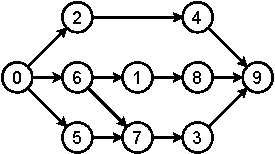
\includegraphics[scale=1.3]{../images/tree.pdf}	
	\column{.45\textwidth} % Left column and width
	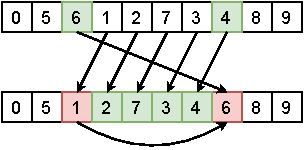
\includegraphics[scale=1.2]{../images/shift0.pdf}
	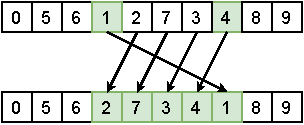
\includegraphics[scale=1.2]{../images/shift1.pdf}	
\end{columns}
\end{frame}

%------------------------------------------------

\begin{frame}
\frametitle{ScheduleMe - Plotter}
\begin{columns}[c] % The "c" option specifies centered vertical alignment while the "t" option is used for top vertical alignment
	
	\column{.45\textwidth} % Left column and width
	\begin{itemize}
		\item Aus Instance .plot Datei schreiben
		\item Kombination aus .rcp und .sol Dateien
		\item Enthält Startzeiten der Aktivitäten und Ressourcenbedarf
		\item Subplot für jede Ressource
		\item Führt Tiefensuche nach zulässiger Darstellung der Lösung aus
		\item Zeichnet Makespan ein
	\end{itemize}
	\column{.45\textwidth} % Right column and width
	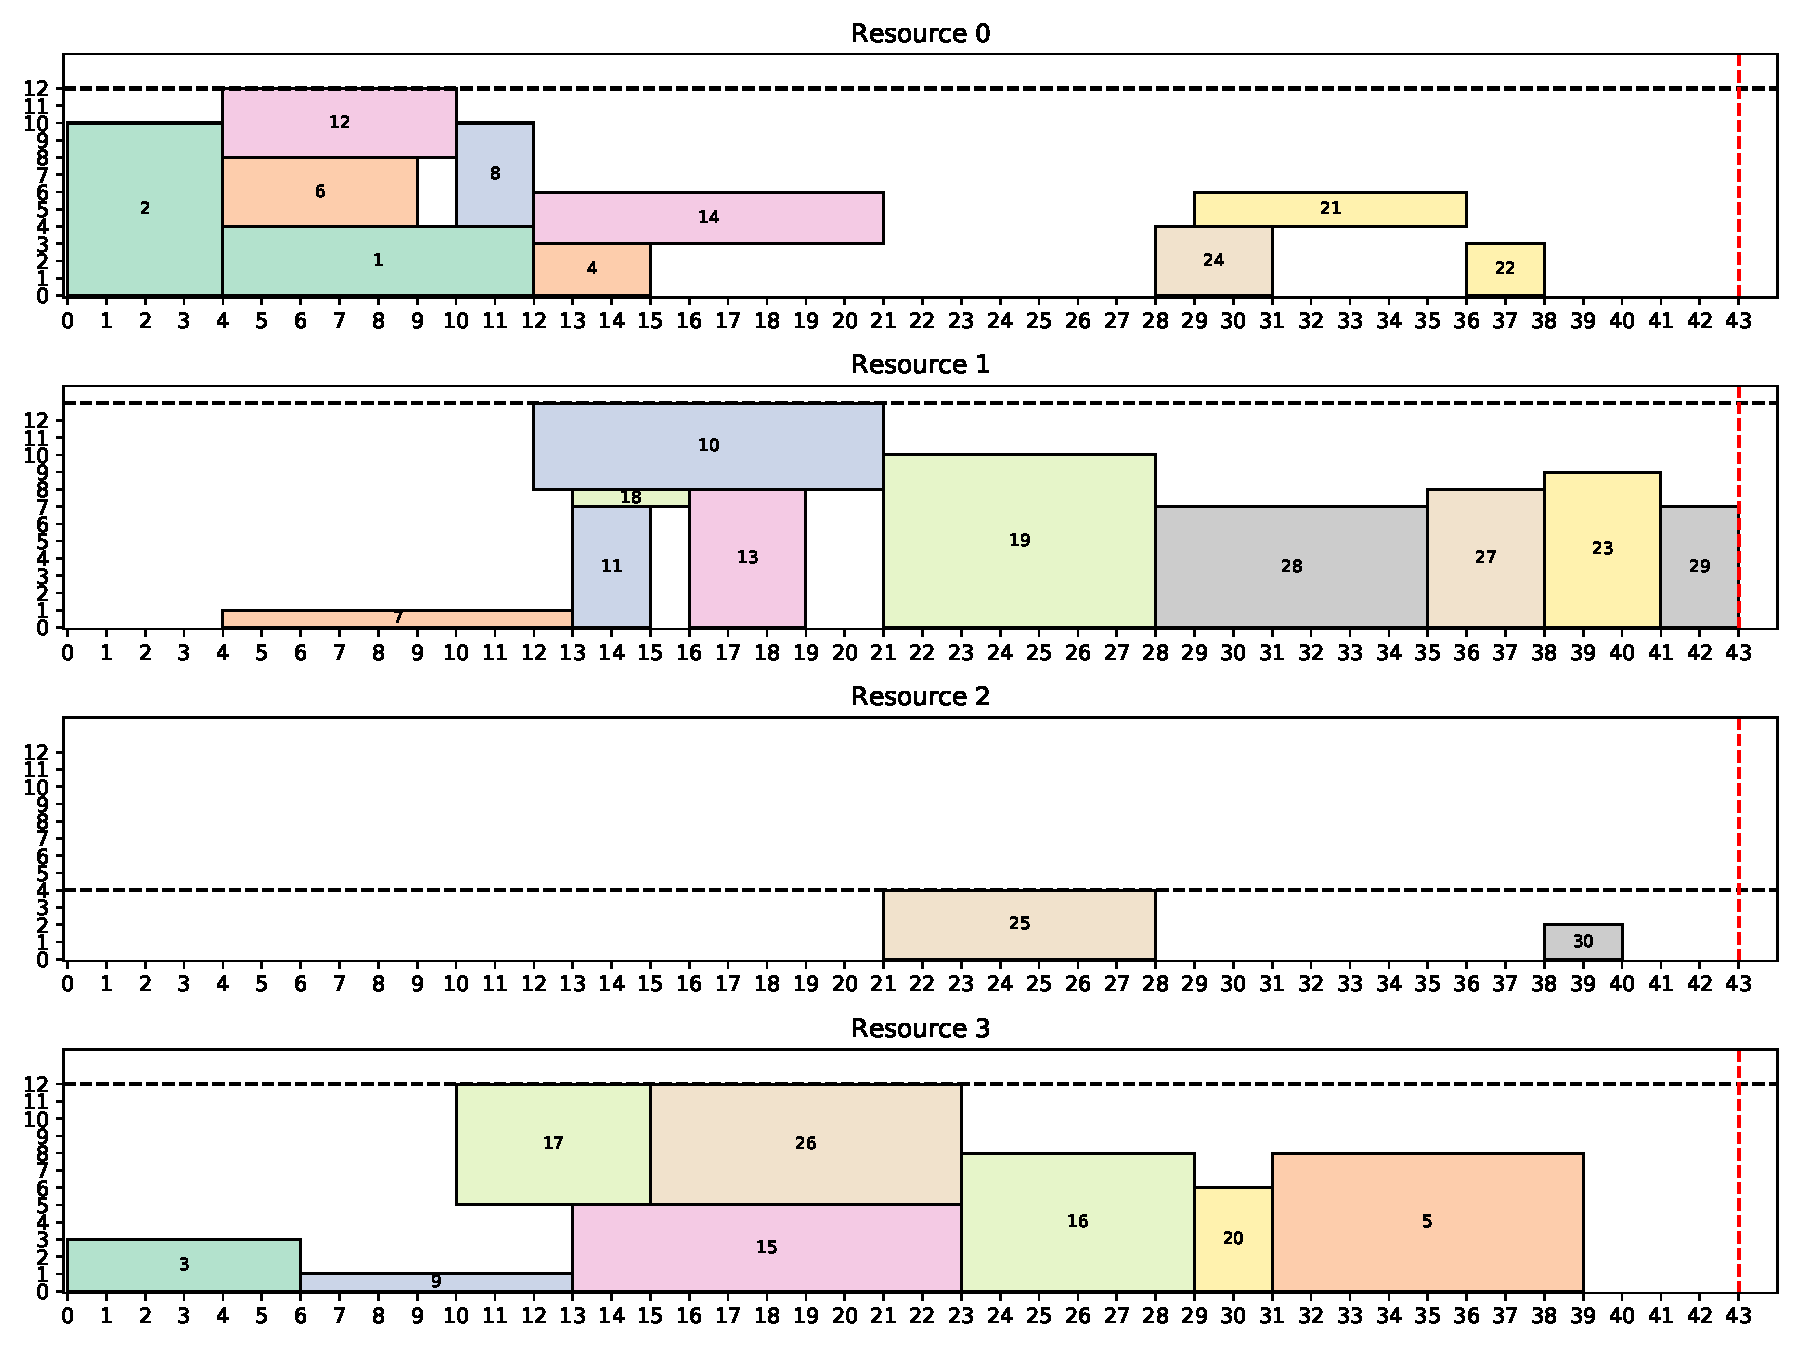
\includegraphics[scale=0.23]{../images/plotter.pdf}		
\end{columns}
\end{frame}

%------------------------------------------------

\begin{frame}
	\frametitle{ScheduleMe - Verbesserung}

	\vspace{-6pt}

	\centering{\small{Instanz J301\_5.RCP}}

	\vspace{-10pt}
	\begin{columns}[c] % The "c" option specifies centered vertical alignment while the "t" option is used for top vertical alignment

		\column{.45\textwidth} % Left column and width

		\centering{\footnotesize{Initial}}
		\vspace{-10pt}

		\begin{figure}
			\centering
			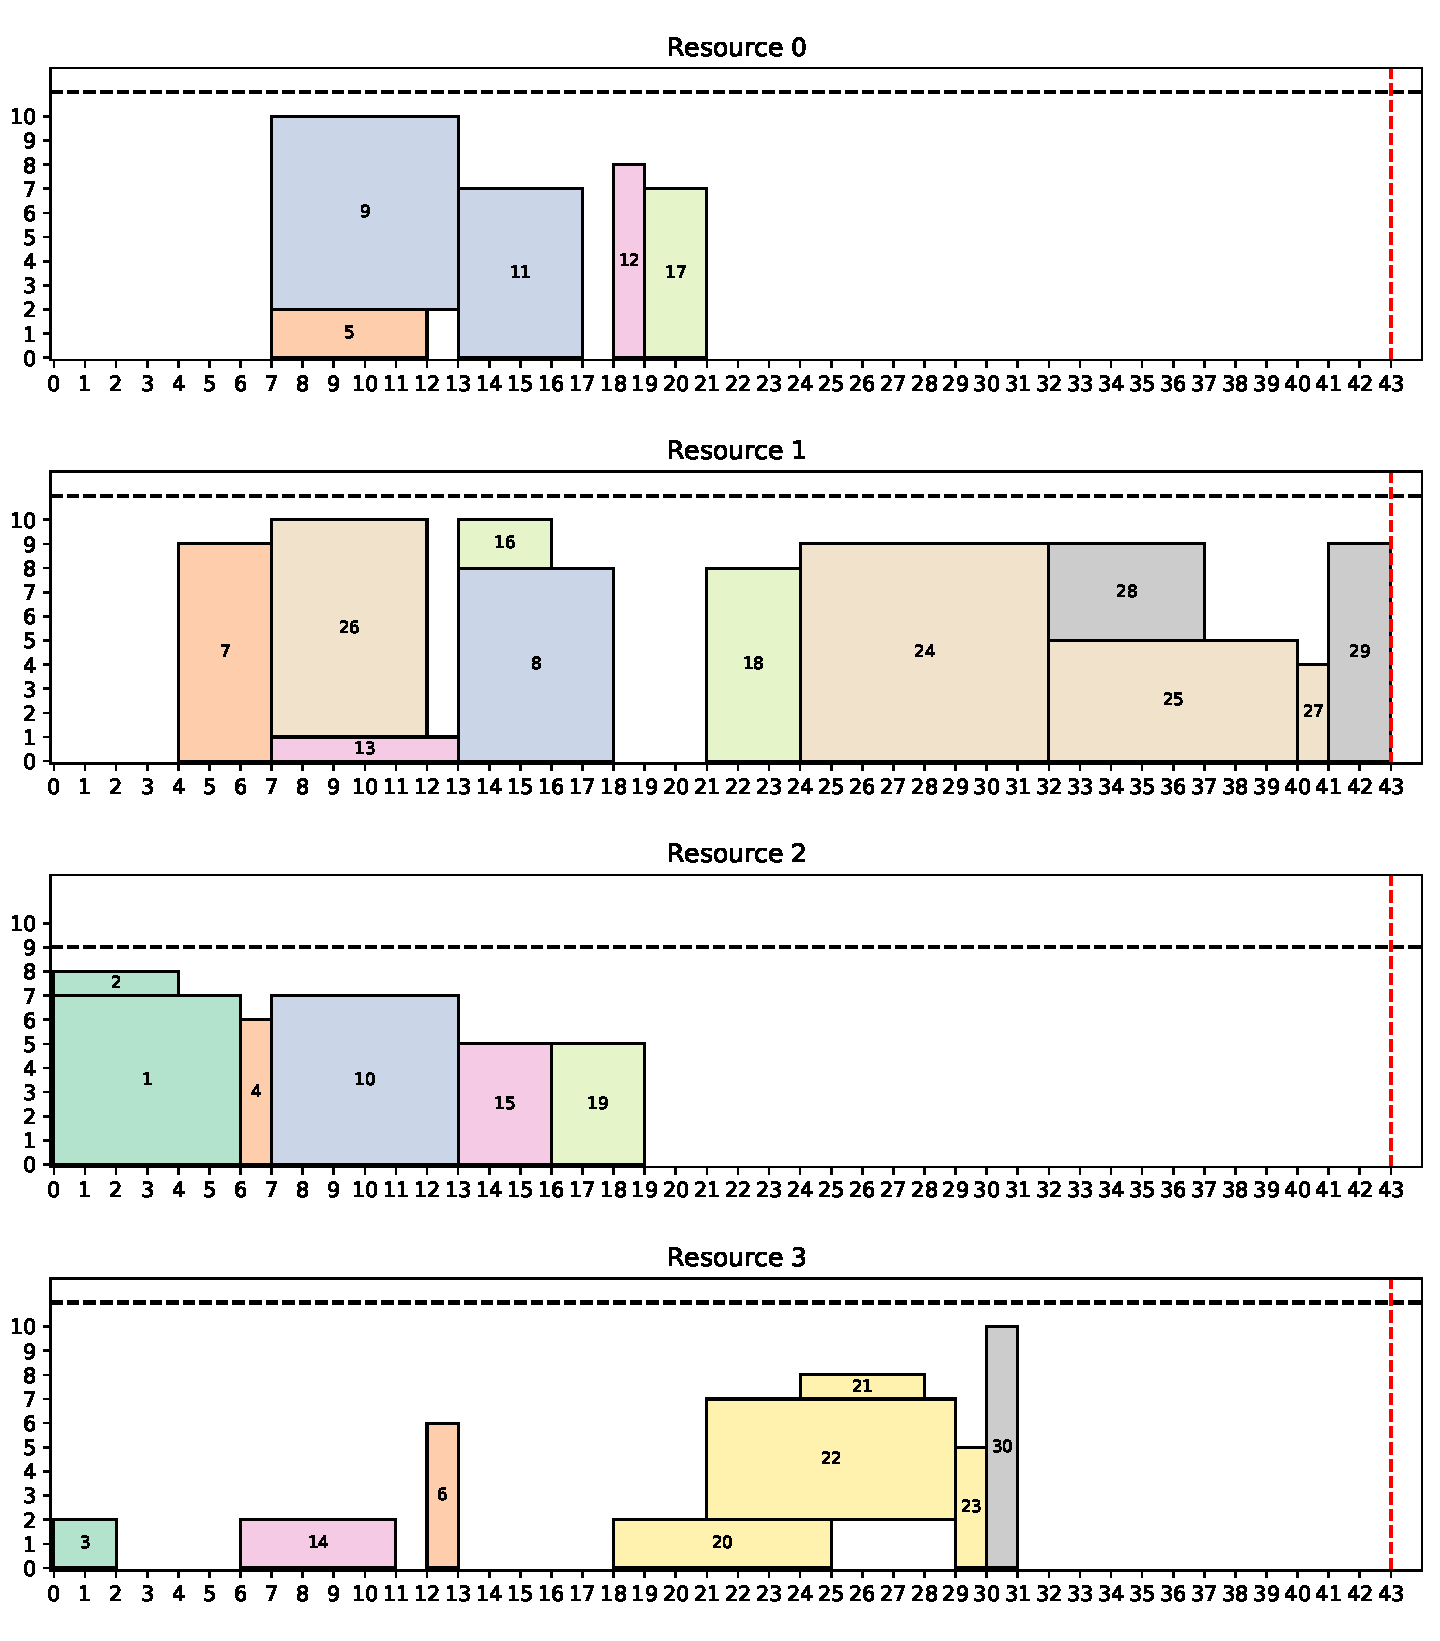
\includegraphics[scale=0.25]{example_plot_init.pdf}
		\end{figure}	
			
		\column{.45\textwidth} % Left column and width

		\centering{\footnotesize{SA SWAP}}
		\vspace{-10pt}

		\begin{figure}
			\centering
			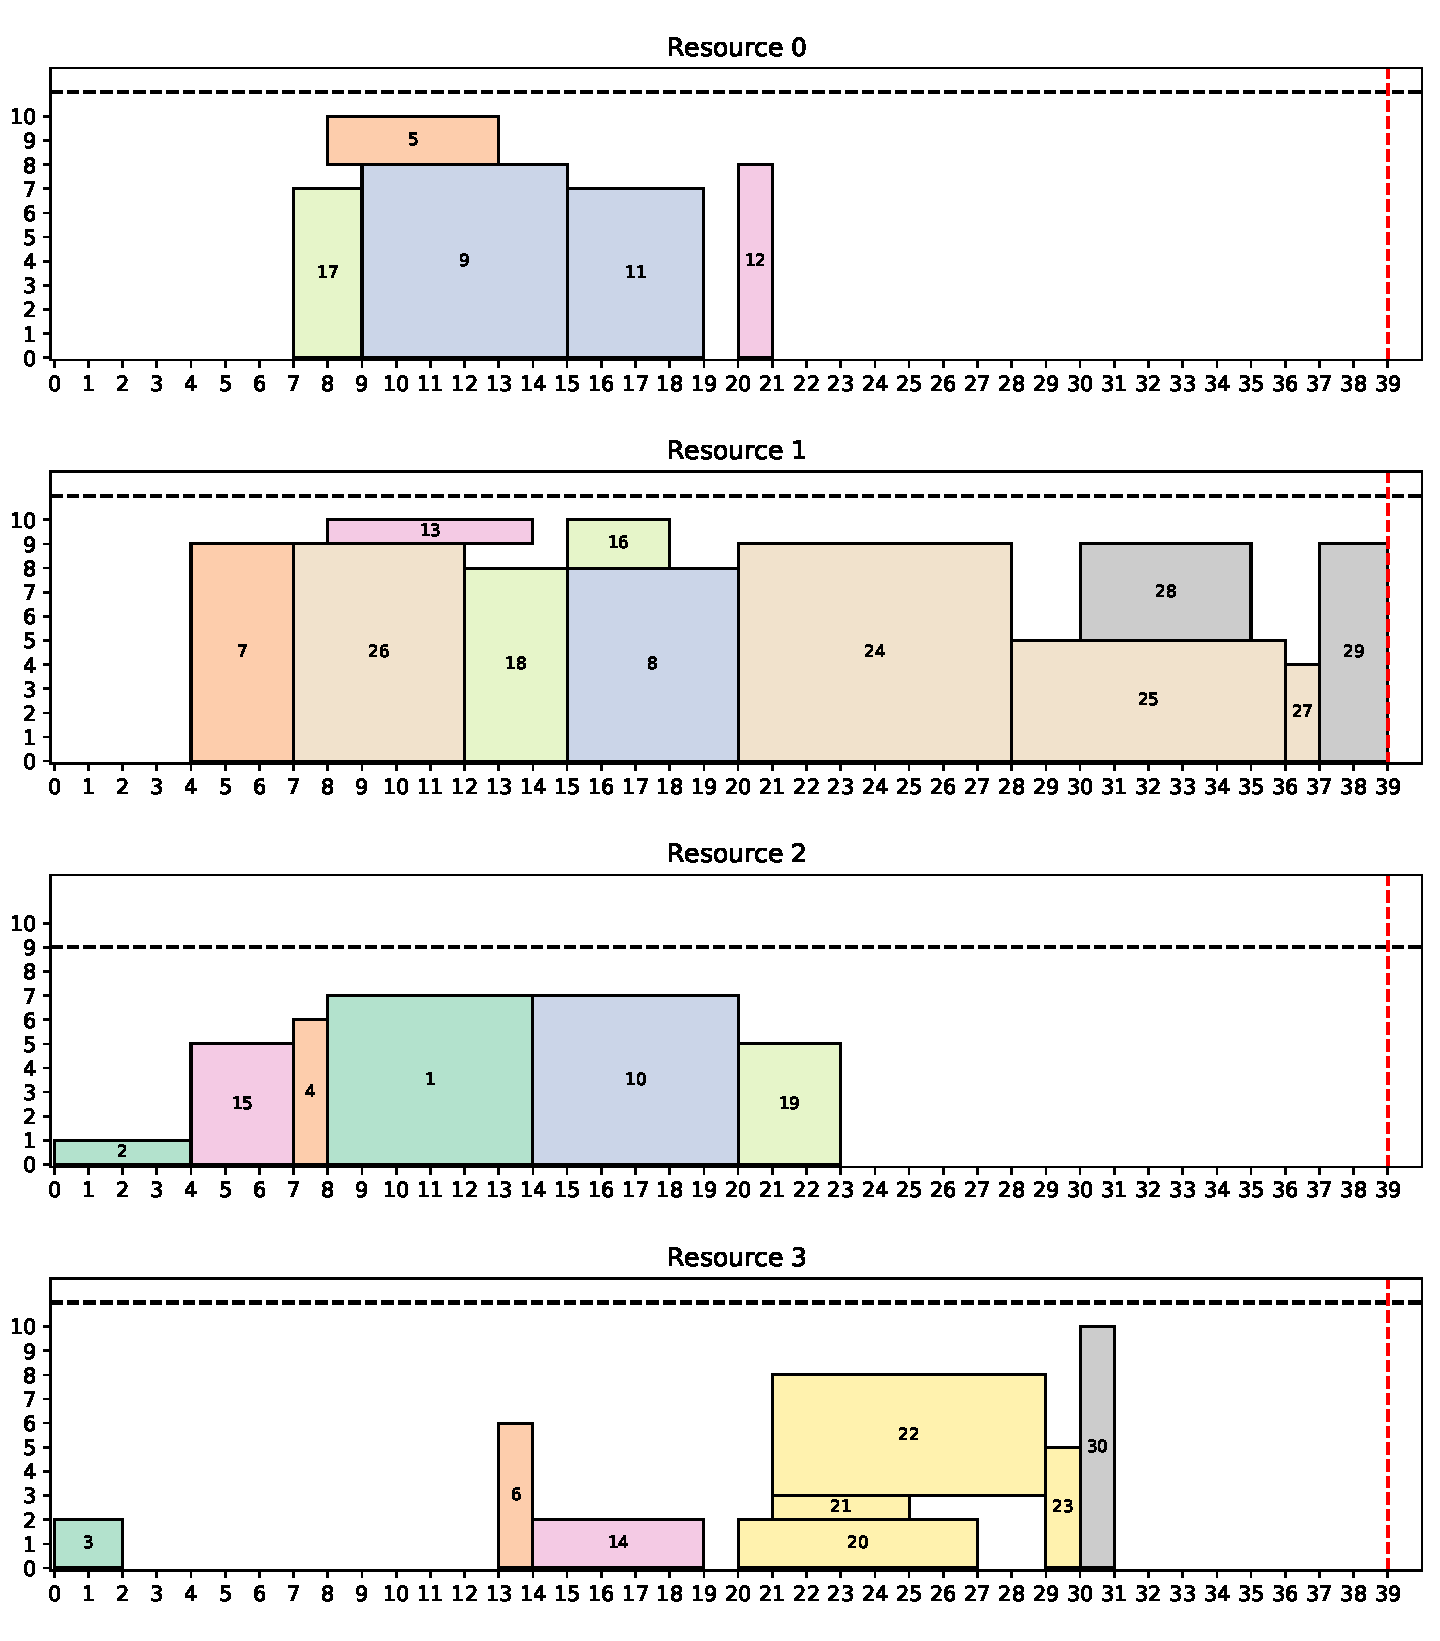
\includegraphics[scale=0.25]{example_plot_sa_swap.pdf}
		\end{figure}	

	\end{columns}
\end{frame}

%------------------------------------------------

\begin{frame}
	\frametitle{ScheduleMe - Vergleich Nachbarschaften}
	
	\vspace{-6pt}
	
	\centering{\small{Instanz J301\_5.RCP}}
	
	\vspace{-10pt}
	\begin{columns}[c] % The "c" option specifies centered vertical alignment while the "t" option is used for top vertical alignment
		
		\column{.45\textwidth} % Left column and width
		
		\centering{\footnotesize{SA API}}
		\vspace{-10pt}
		
		\begin{figure}
			\centering
			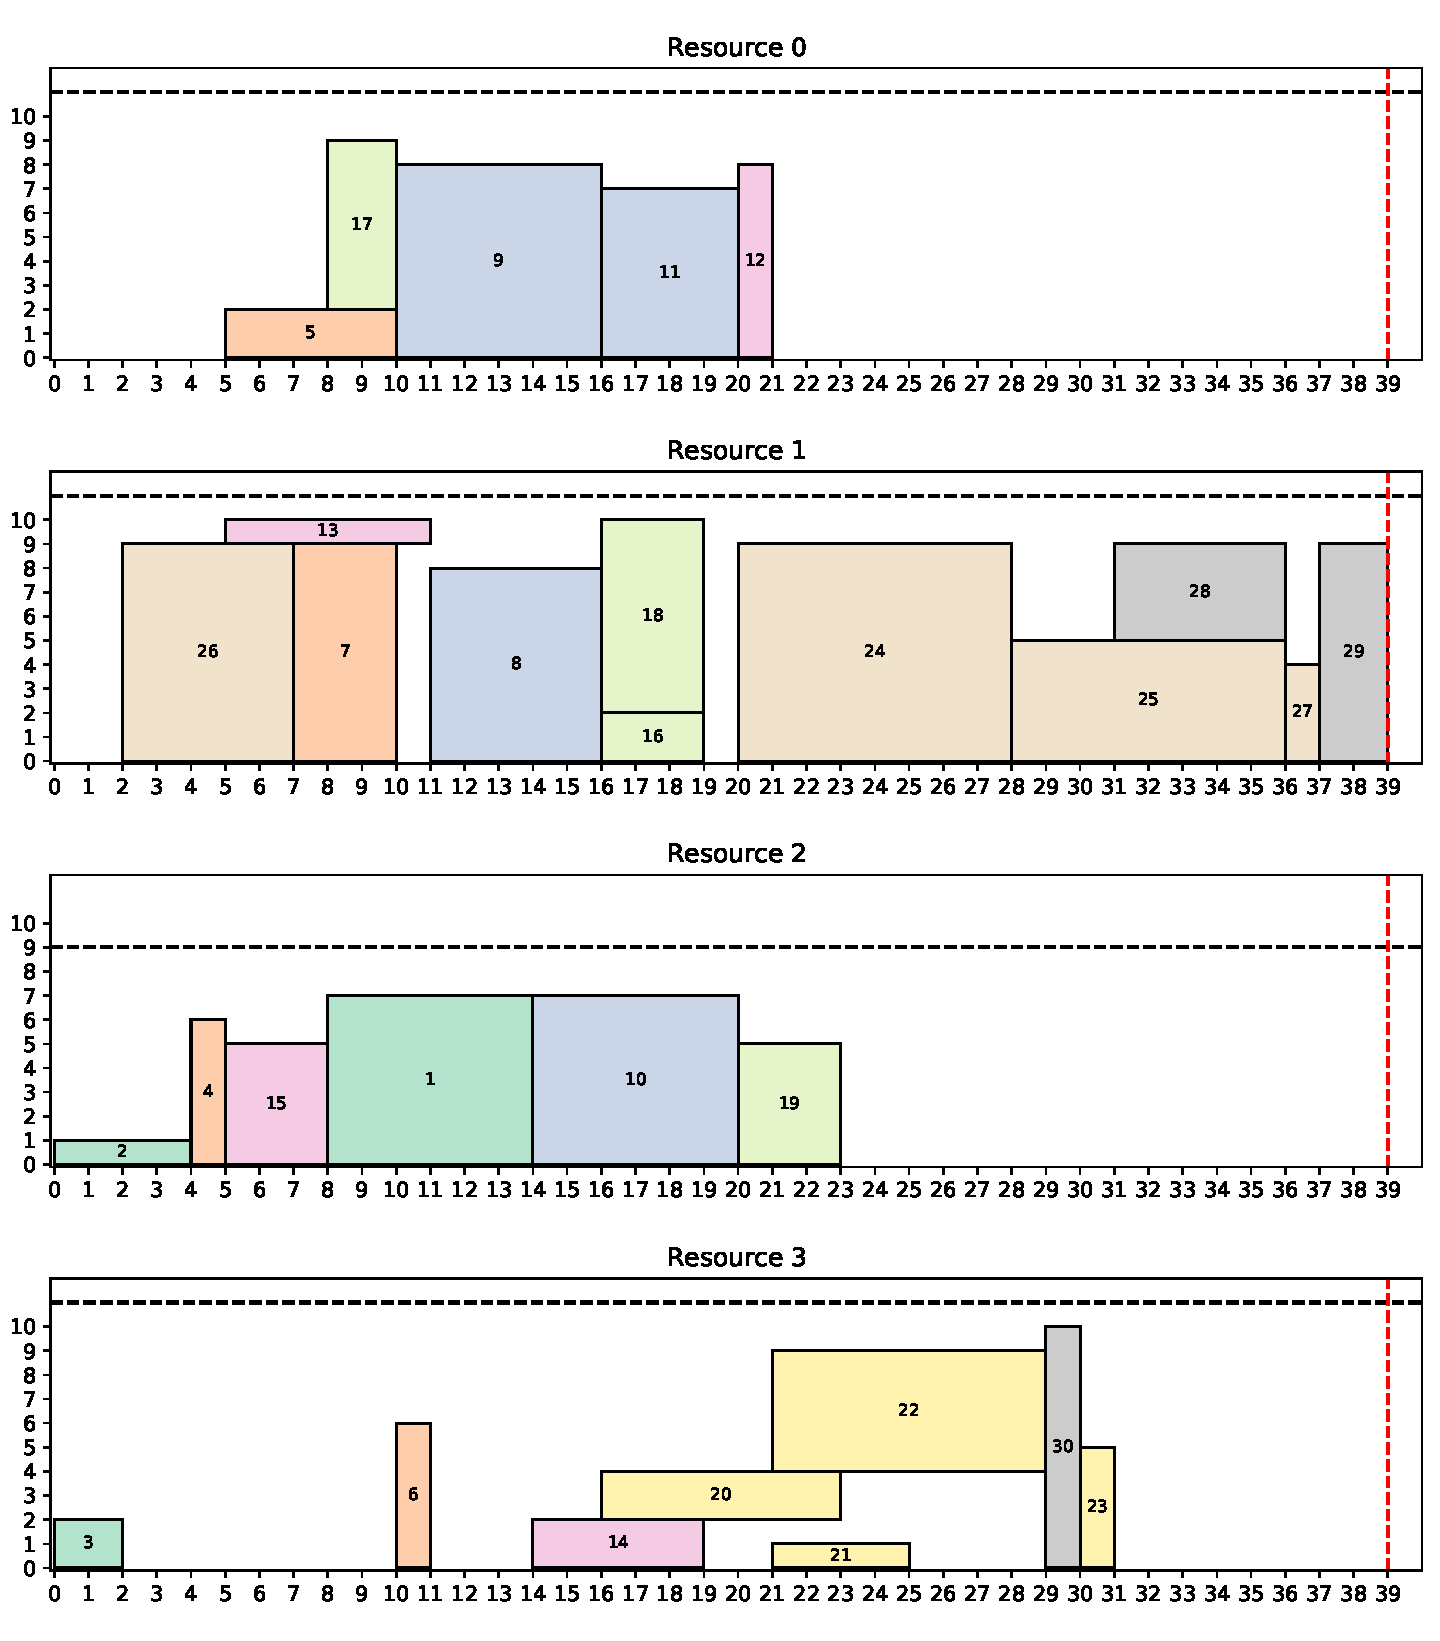
\includegraphics[scale=0.25]{example_plot_sa_api.pdf}
		\end{figure}	
		
		\column{.45\textwidth} % Left column and width
		
		\centering{\footnotesize{SA SWAP}}
		\vspace{-10pt}
		
		\begin{figure}
			\centering
			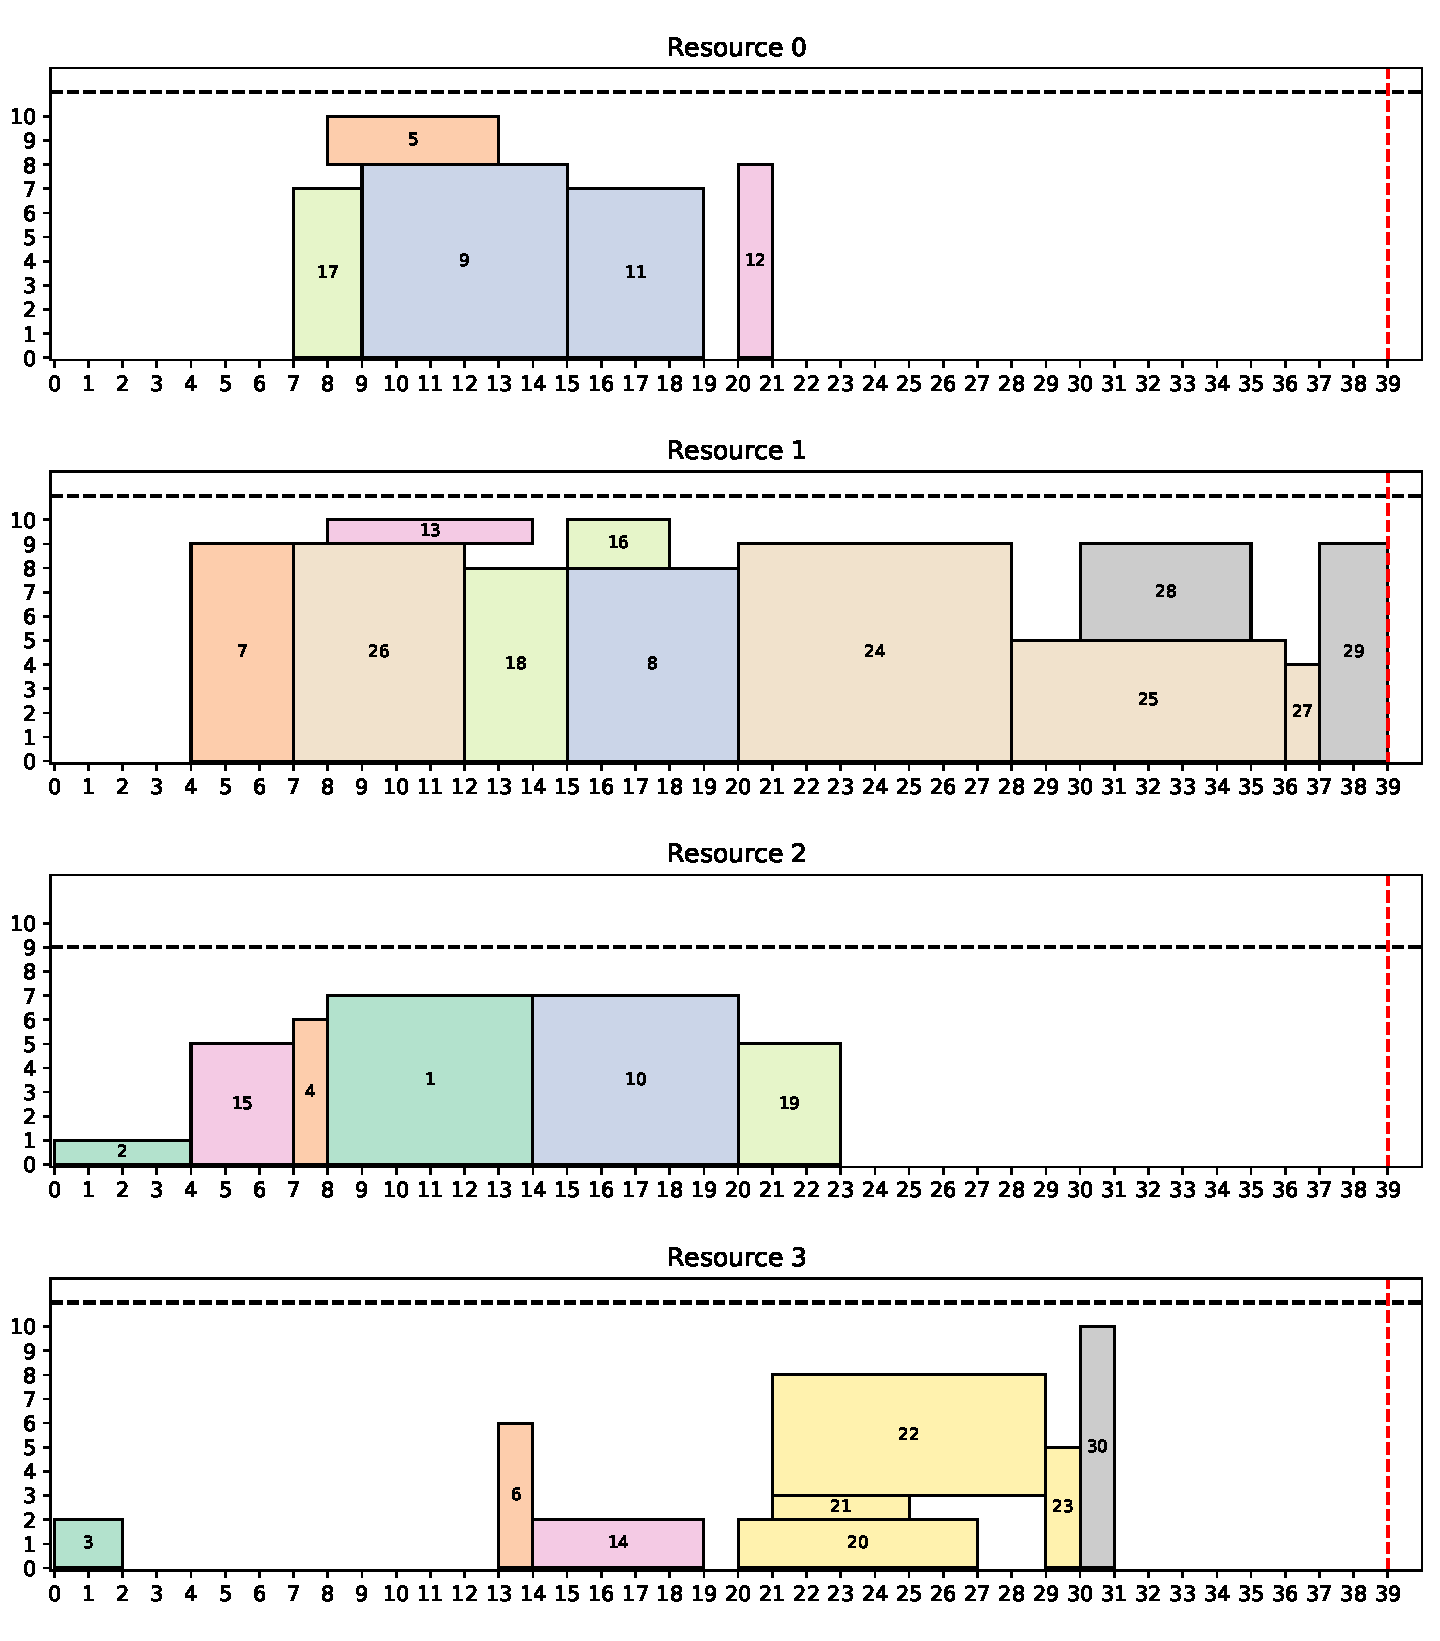
\includegraphics[scale=0.25]{example_plot_sa_swap.pdf}
		\end{figure}	
		
	\end{columns}
\end{frame}

%------------------------------------------------

\begin{frame}[t]
	\frametitle{ScheduleMe - Ergebnisse}
	\vspace{-12pt}
	\begin{figure}
		\centering
		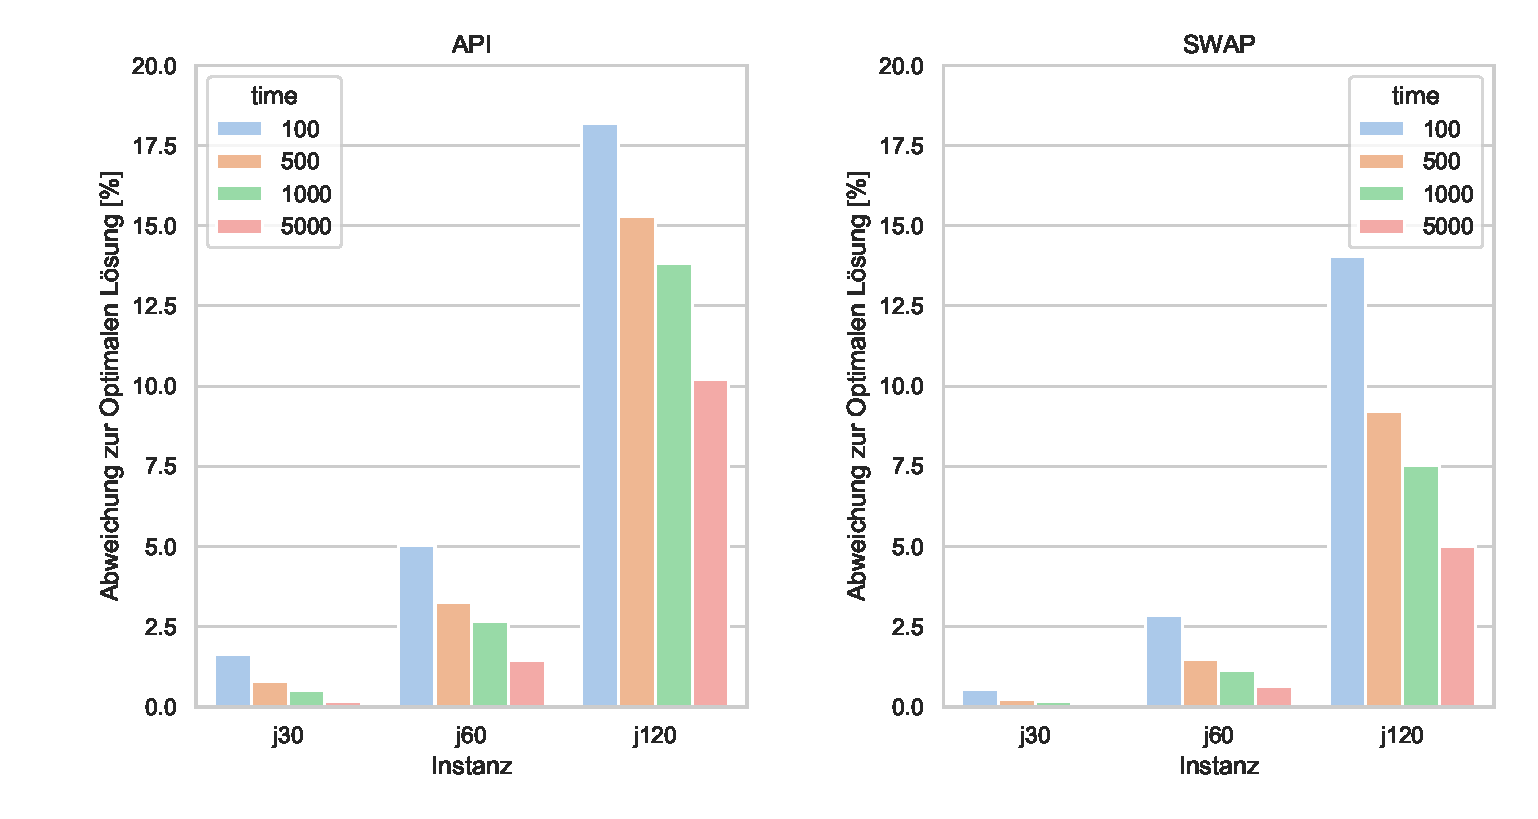
\includegraphics[scale=0.55]{result1.pdf}
	\end{figure}	
\end{frame}

%------------------------------------------------

\begin{frame}[t]
\frametitle{ScheduleMe - Ausblick}

\begin{itemize}
	\item Präzisere Abkühlung durch dynamische Updates von $\alpha$
	\item Andere Nachbarschaften implementieren / testen
	\item Parallelisierung
	\item Laufzeitverbesserung
	\item Anderer Schedule Generation Scheme
	\item Parameter optimieren (Andere Lower Bounds testen)
	\pause
\end{itemize}
\centering
\vspace{40pt}
\textbf{\Large{Fragen?}}
\end{frame}

\end{document} 